\subsubsection*{The Single Responsibility Principle} \label{subsubsec:srp}

The \gls{srp} is one of the fundamental design principles of \gls{ca}. The principle
advocates designing systems with high cohesion and low coupling. The \gls{srp} states that
each module in a system should have only one reason to change. That is, it should have a
single responsibility. No matter the granularity of the module, so implementations of
methods, classes, libraries and/or architecture layers should adhere to \gls{srp}. By
adhering to the principle, each module becomes highly cohesive, meaning that its
responsibilities are closely related and well-defined, while also being decoupled from
other modules \parencite[81]{robert_c_martin_clean_2018}.

\gls{srp} is closely related to the concept of \gls{soc}, which also advocates separating
a system into distinct parts. Although not that clearly stated in the literature,
\citeauthor{robert_c_martin_clean_2018} argues that \gls{soc} intends to have a separation
on a functional level and architectural level. This divides a system into different layers
or components based on their functional roles. \gls{srp} is concerned with separating the
responsibilities of individual modules regardless of the granularity of the module
\parencite[205]{robert_c_martin_clean_2018}.

With this in mind, \gls{srp} adheres more to the definition of \gls{soc} from \gls{ns}.
\textit{A processing function can only contain a single task to achieve stability.} (see
chapter \ref{subsubsec:soc} \nameref{subsubsec:soc}).

There are various manifestations of \gls{srp} implemented in the artifacts. One of which is
already mentioned in Figure \ref{fig:modulair_components}, where \gls{srp} is applied to
separate the domain logic from the application, infrastructure and presentation logic. One
could argue that this manifestation is more related \gls{soc}, considering the high
granularity of the components.

A better example is the separation of handlers that are part of the Clean Architecture
Expander. Each of those handlers executes an isolated part of the expanding process.
Consider the Listing \ref{SipEntityExpander} \nameref{SipEntityExpander}
\parencite{koks_expandentitieshandlerinteractor_2023} for example. This Handler is solely
responsible for the generation of data entities. 

\begin{figure}[H]
    \centering
    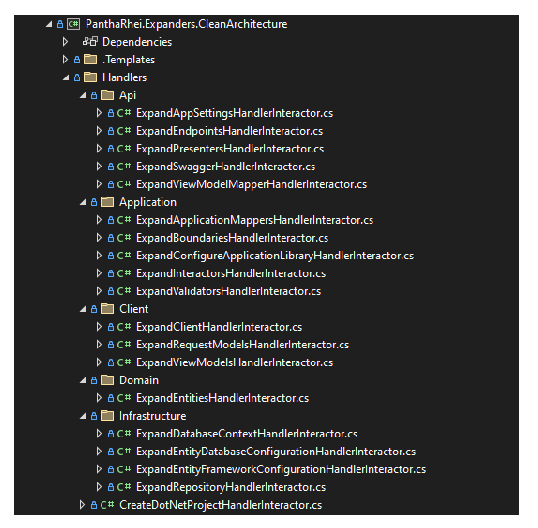
\includegraphics[width=0.7\textwidth]{Figures/expander_handlers.pdf}
    \caption[handlers]{Each of the handlers handles an isolated part of the expanding process.}
    \label{fig:handlers}
\end{figure}

\lstinputlisting[
    caption={The \citetitle{koks_expandentitieshandlerinteractor_2023}},
    label={SipEntityExpander}]
    {Snippets/ExpandEntitiesHandlerInteractor.cs}